\documentclass[pdftex, 11pt, a4paper, titlepage]{article}
\usepackage[slovak]{babel}
\usepackage[utf8]{inputenc}
\usepackage[IL2]{fontenc}
\usepackage[left=2.5cm, top=2.5cm, text={16.5cm, 25cm}]{geometry}
\usepackage{graphicx}
\usepackage{amsmath}
\usepackage{mathtools}
\usepackage{hyperref}
\usepackage{alltt}

\newcommand{\code}{\texttt}

\begin{document}
    \begin{center}
        \section*{Umělá inteligence pro Válku kostek}
        \subsection*{VUT Fakulta Informačních Technologií v Brně}
        \subsection*{SUI 2021/2022}
        \begin{tabular}{ r l l }
            Autori: & {Matej Záhorský} & \texttt{xzahor04} \\
            & {Matúš Škuta} & \texttt{xskuta04} \\
            & {Patrik Németh} & \texttt{xnemet04}
        \end{tabular}
    \end{center}

    \section{Princíp hry}
    Pre kontext sa v krátkosti uvedie princíp hry.
    Hra Dicewars spočíva v dobíjaní území hracej plochy rozdelenej medzi zúčastnených hráčov. Územia obsahujú hracie kocky, pričom každé územie ich obsahuje
    minimálne jednu a maximálne osem. Pri dobíjaní územia sa \uv{hodí} kockami z dvoch území, ktoré sa zúčastňujú bitky. Ak útočníkov súčet hodnôt hodených kociek
    je vyšší, než obrancov, útočník obsadzuje. Ak je nižší alebo rovný ako obrancov súčet, tak sa neobsadzuje, útočník stráca všetky kocky a obranca stráca
    kocky dané vzťahom $\lfloor \frac{\text{počet kociek útočníka}}{\text{4}} \rfloor$. Vyhráva hráč, ktorý obsadí celú hraciu plochu.

    \section{Implementácia}
    Implementácia hráča s umelou inteligenciou (ďalej iba \emph{bot}) je zameraná na prehľadávanie stavového priestoru pomocou Alfa-Beta algoritmu,
    rozhodovanie o optimálnosti útoku pomocou neurónovej siete a na prehľadávanie priestoru hracej plochy za účelom vhodných podporných presunov kociek.
    Jedno kolo bota je rozdelené na tri možné fázy: \textbf{útok}, \textbf{obrana}, \textbf{presun}. Poradie týchto fáz sa nemení, avšak je možné preskočiť prvú fázu,
    prípadne nevykonať ani jednu. Rozhodnutie o prípadnom preskakovaní fáz je vykonané na začiatku každého kola na základe výstupu Alfa-Beta algoritmu.

    \subsection{Fázy kola}
    Správanie bota je dané súčasnou fázou kola, v ktorom sa bot nachádza. Bot je inicializovaný do fázy útoku a do tejto fázy sa vracia na konci každého kola
    pred vydaním príkazu \code{EndTurnCommand}.

    \subsubsection*{Útok}
    V prípade \emph{úplného} kola, teda kola, v ktorom sa nepreskakujú fázy, sa najprv volá metóda\\ \code{AI.get\_attack()}. Táto metóda vyhľadáva útoky, ktoré:
    \begin{itemize}
        \item je možné vykonať bez podporných presunov,
        \item je možné vykonať s podpornými presunmi, ktoré:
        \begin{itemize}
            \item podporujú útok,
            \item podporujú obranu po útoku.
        \end{itemize}
    \end{itemize}
    Vyhodnotenie rozhodujúce o optimálnosti útoku poskytuje v metóde \code{AI.get\_attack()} trénovaná neurónová sieť (viac v sekcii \ref{sec:nn}).
    V prípade, že padne rozhodnutie o vykonaní útoku, pozbierajú sa prípadné podporné presuny, ktoré sa vykonajú v danom poradí
    (teda presuny podporujúce útok sa vykonajú pred útokom a presuny podporujúce obranu sa vykonajú po útoku). Počet týchto podporných presunov je obmedzený
    na štyri.

    \subsubsection*{Obrana}
    Ďalšou fázou je fáza obrany. Vzhľadom na princíp hry je vhodné byť do istej miery agresívny. Avšak napriek tomu, že sa útoky vykonávajú iba v prípade vysokej
    udržateľnosti prípadného rozšíreného územia, je nutné ochrániť už vlastnené územie v reakcii na zmenu stavu hry zo strany nepriateľov.
    Metóda \code{AI.gen\_deffense\_moves()}\footnote{Slovo \uv{defense} je v zdrojovom kóde na niektorých miestach omylom písané s dvojitým \uv{f}.}
    generuje obranné presuny s prioritou obrany najslabších území na hraniciach regiónov. Maximálny počet týchto presunov za kolo nie je obmezdený.

    \subsubsection*{Migrácia}
    V prípade, že po obrannej fáze vystanú presuny pre dané kolo, vykonajú sa \uv{migračné} presuny. Význam týchto presunov je udržiavať čo najviac
    kociek v dosahu území, ktorých okolie je najslabšie. Toto sa vyhodnocuje na základe rozdielu súčtov priateľských a nepriateľských kociek v susedstve
    vyhodnocovaného územia na hranici regiónu. Kocky migrujú buď z území, ktoré sú čo najbližšie k hraniciam (v prípade, že vlastníme menej, než polovicu hracej plochy),
    prípadne z území, ktoré sú najďalej od hraníc (v prípade, že vlastníme vyše polovicu hracej plochy). Tieto presuny generuje metóda \code{AI.gen\_transfer\_moves()}.

    \subsection{Alfa-Beta algoritmus}
    Na začiatku každého kola sa spustí algoritmus Max\textsuperscript{n} s Alfa-Beta orezávaním\footnote{KORF, Richard E. Multi-player alpha-beta pruning. \emph{Artificial Intelligence}. Elsevier. 1991, zv. 48, č. 1, s. 99-111.}.
    Prehľadávanie sa mimo nášho ťahu vykonáva do hĺbky 3, čo činí jedno kolo pre každého hráča. Algoritmus sa spúšťa v metóde \code{AI.alpha\_beta\_entry()},
    ktorá následne volá rekurzívnu verziu \code{AI.alpha\_beta()}. Každý uzol stromu prehľadávania generuje tri podstromy podľa spôsobu vykonania súčasného kola.
    Spôsoby vykonania kola sú: úplné kolo, preskočenie fázy útoku a žiadna akcia. Pre každý spôsob vykonania kola sa rekurzívne volá Alfa-Beta algoritmus, ktorý
    vracia vyhodnotenie hracej plochy na základe počtu obsadených území jednotlivými hráčmi, teda maximalizovanou hodnotou je počet vlastnených území.

    Simulácia jednotlivých kôl prebieha v metóde \code{AI.simulate\_turn()}, ktorá vykonáva zjednodušenú simuláciu priebehu kola (vlastne sa jedná o prispôsobený
    kód z modulu \code{dicewars.server.game}). Po simulácii každého spôsobu vykonania kola sa rekurzívne volá Alfa-Beta na simulovanú hraciu plochu.
    Po návrate z rekurzie sa simulovaná hracia plocha vráti do pôvodného stavu metódou \code{AI.unsimulate\_turn()}.

    \subsection{Neurónová sieť}\label{sec:nn}
    Model neurónovej siete je založený na neurónovej sieti učiacej sa hrať hru Snake\footnote{Odkaz na github repozitár: \href{https://github.com/python-engineer/snake-ai-pytorch}{https://github.com/python-engineer/snake-ai-pytorch}.},
    ktorá bola prispôsobená účelom projektu. Jej cieľom je odhadovať, či je nejaké územie udržateľné naprieč jednou rotáciou kôl po ukončení kola bota -
    teda vracia rozhodnutie, či územie spolu s jeho kockami okamžite nestratíme.

    Pred zistením udržateľnosti územia sa najprv útok odsimuluje ako úspešný\footnote{Stav pred útokom nemá vplyv na rozhodovanie neurónovej siete, čiže týmto sa zvýši počet trénovacích dát.},
    vykoná sa predikcia a následne je uložený aktuálny stav hry, ktorý sa neskôr použije na trénovanie neurónovej siete. Stav hry je definovaný ako počet kociek územia,
    ktorého udržateľnosť testujeme, následne počet kociek nanajvyš piatich najsilnejších susedných nepriateľských území, ktoré sú zoradené zostupne a nakoniec
    vlastníctvo územia, ktoré je síce v čase predikcie vždy rovnaké, ale môže sa zmeniť na základe akcií protivníkov. Okrem stavu hry pred akciou sa na trénovanie
    využívajú informácie o stave hry po vykonaní akcie, o danej akcii a odmene. Po vykonaní vybranej akcie sa buď pokračuje ďalej, alebo ukončuje ťah.
    Následne je na začiatku každého kola vykonávané trénovanie neurónovej siete. Pre trénovanie sa získa nový stav hry každej oblasti,
    pre ktorú sme vykonali predikciu v minulom ťahu a na základe korektnosti predikcie sa neurónovej sieti udelia odmeny (správna predikcia činí pozitívnu odmenu,
    nesprávna predikcia činí negatívnu odmenu). Keďže sa týchto akcii za ťah môže vykonať viac, získavame nový stav pre každú predikciu, uďelujeme
    odmeny a trénujeme sieť až do bodu, keď predikcie začnú byť vo väčšine prípadoch správne.

    \section{Priebežné vyhodnocovanie implementácie}
    Vyhodnocovanie prebiehalo so zvyšujúcimi sa nárokmi na úspešnosť voči vždy obtiažnejším súperom. Prvé iterácie umelej inteligencie boli testované proti
    botom \code{dt.ste}, \code{dt.stei} a \code{kb.sdc\_post\_dt}. Zpočiatku bolo cieľom poraziť najslabšieho bota z tých, proti ktorým bude
    vyhodnocovaný (podľa zadania). Zakaždým keď sa botovi podarilo výrazne zlepšiť, tak sa najslabší bot nahradil ďalším v poradí z testovacích botov.
    Výrazným prínosom bolo posilňovanie útokov a prípadné dodatočné posilnenie území po útoku pomocou presunov.
    Neurónová sieť prešla niekoľkými iteráciami funkcie generujúcej odmeny. Ako výsledná bola zvolená tá, ktorá robila najmenšie chyby v predikciách.

    \section{Záver}
    Bot má v súčasnej verzii vysokú úspešnosť voči \code{dt.stei} a \code{kb.stei\_dt}. Na základe testovania s fixným poradím hráčov na 1000 hracích plochách
    je implementovaný bot na približne rovnakej úrovni ako \code{kb.sdc\_pre\_at}. Na grafe konvergencie víťazstiev (viď obrázok \ref{obr:graf})
    je však od neho badateľne slabší. Predpoklad je, že pri štatisticky reprezentatívnejšom počte hier sa počty víťazstiev vyrovnajú.

    \begin{figure}[h]
        \centering
        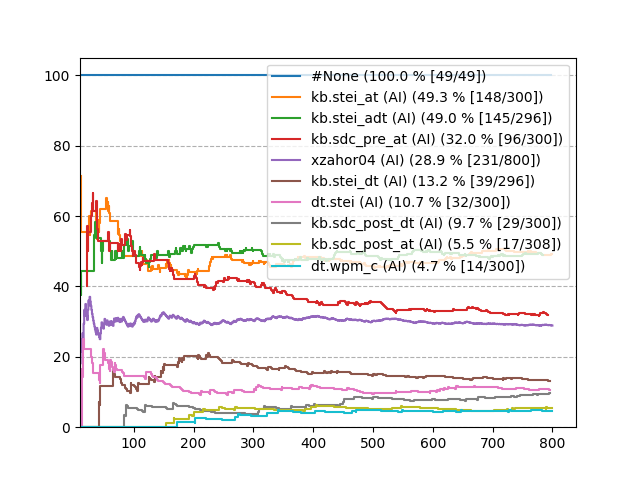
\includegraphics[scale=0.85]{tournament_plot.png}
        \caption{Graf konvergencie víťazstiev v hrách štyria proti štyrom na 200 rôznych hracích plochách.}
        \label{obr:graf}
    \end{figure}

    \subsection{Známe nedostatky a možné vylepšenia}
    V prvom rade je potrebné reorganizovať, refaktorizovať a zjednodušiť zdrojový kód. Alfa-Beta algoritmus nie je vylepšený, aby efektívnejšie prerezával podstromy.
    Vyhodnocovacia funkcia využívaná pri prehľadávaní stavového priestoru by mala zohľadňovať aj defenzívnu silu regiónov jednotlivých hráčov.

\end{document}